\subsubsection{26.03.15}

Today we had a flight to Amsterdam trough Frankfurt. Next we went to Eindhoven (the town where the competition takes place) by train. Then we settled into the hoteland started working on robot.

\begin{enumerate}
	
	\item The time of beginning and ending of the meeting: 12:00 - 23:59.
	
	\item Purposes of the meeting: 
	\begin{enumerate}
		
		\item Reassemble robot after transportation.
		
		\item Finish the mechanism of overturning of the bucket and fix it on the robot.
		
		\item Install the plexiglass protection onto the robot.
		
        \item Connect servos from the bucket overturner to the controllers.
        
        \item Prepare for the presentation of the engineering book to the judges at the competition.
		
	\end{enumerate}

	\item Work that has been done:
	\begin{enumerate}
		
		\item At first, we reassembled robot from parts.
		
		\item Next we pasted stickers to the plexiglass protection and then fixed it on the robot.
		\begin{figure}[H]
			\begin{minipage}[h]{0.47\linewidth}
				\center{
\includegraphics[scale=0.5]{days/26.03.15/images/01}}
			\end{minipage}
			\hfill
			\begin{minipage}[h]{0.47\linewidth}
				\center{
\includegraphics[scale=0.8]{days/26.03.15/images/02}}
			\end{minipage}
			\caption{Stickers for the plexiglass}
		\end{figure}
		
        \item We finished working on mechanism of overturning of the bucket. Next it was installed to the last pair of slats. The gutter for balls and the bucket were fixed on this module. Now the bucket overturner is working stable and looks more reliable than it was before.
        \begin{figure}[H]
        	\begin{minipage}[h]{0.47\linewidth}
        		\center{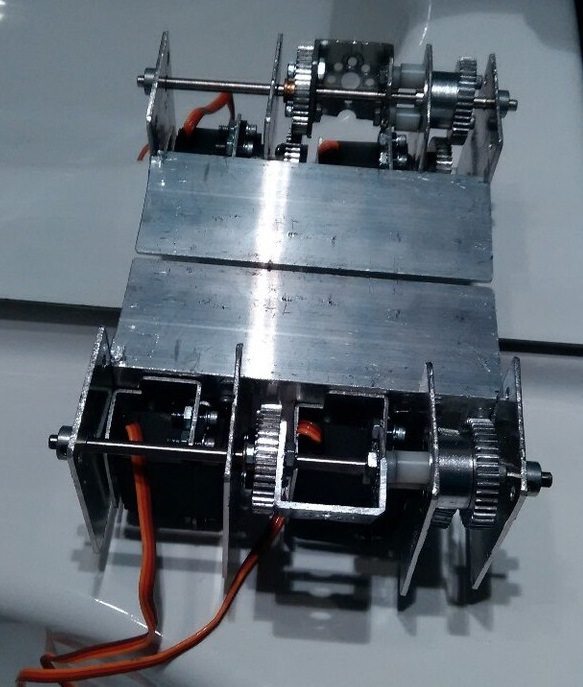
\includegraphics[scale=0.25]{days/26.03.15/images/03}}
        		\caption{Stickers for the plexiglass}
        	\end{minipage}
        	\hfill
        	\begin{minipage}[h]{0.47\linewidth}
        		\center{
\includegraphics[scale=0.3]{days/26.03.15/images/04}}
        		\caption{Stickers for the plexiglass}
        	\end{minipage}
        \end{figure}
        
        \item The mount of axis on the last pair of slats on elevator was moved 16 mm up because it beated the motor at the bottom position.
        
        \item To connect the servos from the bucket overturner to the controllers we decided to create a system that we had seen in Moscow on some robots. We made the additional lift - a number of beams, connected to each other with hinges like a chain. The first beam was connected to the carcase of the robot and the last one - to the top of the main lift. The wire was fixed on these beams, so there was no risk of entanglement. We refused our previous solution with fixing the wire on the main lift because there were problems. The bucket was always clinging the wire and bicket couldn't go to the bottom, so it disturbed scoring balls into the bucket.
        \begin{figure}[H]
        	\begin{minipage}[h]{0.2\linewidth}
        		\center  
        	\end{minipage}
        	\begin{minipage}[h]{0.6\linewidth}
        		\center{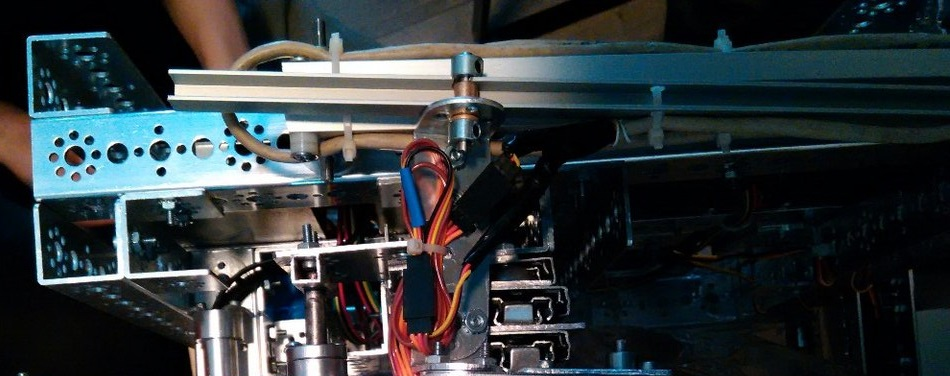
\includegraphics[scale=0.3]{days/26.03.15/images/05}}
        		\caption{}
        	\end{minipage}
        \end{figure}
        
        \item After we finished all works with construction, we rehearsed the presentation of our engineering documentation.
		
        

	\end{enumerate}
	
	\item Results:
	\begin{enumerate}
			
			\item Robot was reassembled after transportation.
			
			\item The mechanism of overturning of the bucket was finished and installed on the robot.
			
			\item The plexiglass protection was fixed on the robot.
			
			\item Servos from the bucket overturner were connected to the controllers with additional lift.
			
			\item Prepare for the presentation of the engineering book to the judges at the competition.
			
	\end{enumerate}
	
	\item Tasks for the next meetings:
	\begin{enumerate}
		
		\item Realise opening of the mechanism for directing balls vertically.
		
		\item Prepare autonomus programs.
			
	\end{enumerate}
\end{enumerate}
\fillpage
